\section{Experiments}
\label{sec:results}

We evaluate CAPO on a controlled RLVR setting designed to isolate the effect of
advantage aggregation. All results are produced with a single open-weight model
(Qwen2.5--1.5B--Instruct) and a single task distribution (CountDown).

\subsection{Setup}
\paragraph{Task.} CountDown presents a target integer and a small multiset of
integers; the model must return an arithmetic expression that evaluates to the
target. We use the standard exact-match verifier, yielding a binary outcome
reward.

\paragraph{Model.} We finetune Qwen2.5--1.5B--Instruct with group-based
on-policy RL. For each prompt, we sample $N=8$ trajectories per update, matching
the aggregation dimension assumed by GRPO-style estimators.

\paragraph{Context budgets.} We report two response-length regimes:
(i) a \emph{short} regime with maximum response length 2048 tokens and
(ii) a \emph{long} regime with maximum response length 8192 tokens. Unless
otherwise noted, all other hyperparameters are kept identical across regimes.

\paragraph{Implementation.} We implement all methods within the same training
stack (VERL), holding fixed the rollout procedure, optimizer, and training
schedule. This ensures that differences can be attributed to the advantage
aggregation / normalization rule rather than to unrelated systems choices.

\paragraph{Group-based objective and estimator.}
All baselines and CAPO variants use the same group-based on-policy objective.
Concretely, for each prompt we sample $N$ trajectories, compute token-level policy-gradient terms using the same clipping and advantage conventions, and differ only in how the per-trajectory advantages (and hence token-level losses) are reweighted as a function of trajectory length and dependence.
This isolates the effect of the aggregation rule discussed in \S\ref{sec:setup}--\S\ref{sec:method}.

\paragraph{Hyperparameters and reproducibility.}
We use identical optimizer, rollout, and training-schedule hyperparameters across all methods within a given context budget.
For transparency and reproducibility, we report the key optimization hyperparameters in Table~\ref{tab:hyperparams}.
Unless otherwise stated, all reported curves are averaged over multiple random seeds; the stability metrics in Table~\ref{tab:stability} are computed from the per-seed validation trajectories prior to averaging.

\begin{table}[t]
\centering
\small
\begin{tabular*}{\textwidth}{@{\extracolsep{\fill}}ll}
\toprule
Hyperparameter & Value \\
\midrule
Base policy model & Qwen2.5--1.5B--Instruct \\
RL stack & VERL \\
Task / reward & CountDown verifier (binary success) \\
Trajectories per prompt ($N$) & 8 \\
Max response tokens & $\{512, 1024, 2048\}$ \\
Optimizer & \textemdash \\
Learning rate & \textemdash \\
PPO/GRPO cliprange & \textemdash \\
Rollout temperature & \textemdash \\
Prompts per update ($M$) & \textemdash \\
Evaluation frequency & \textemdash \\
Random seeds & \textemdash \\
\bottomrule
\end{tabular*}

\caption{Key optimization and rollout hyperparameters used in the CountDown RLVR experiments.
We hold these fixed across methods within a given context budget; only the advantage aggregation / normalization rule varies.}
\label{tab:hyperparams}
\end{table}

\subsection{Baselines and method variants}
We compare CAPO against a set of aggregation baselines that progressively add
or remove normalizations:
\begin{itemize}
  \item \textbf{DAPO normalization} (token-mean): GRPO with token-averaged policy
  loss.
  \item \textbf{GRPO normalization} (seq-mean-token-mean): GRPO with per-sequence
  normalization of the loss, which empirically reduces length bias but can
  increase variance.
  \item \textbf{Dr.~GRPO normalization:} GRPO with distributional-reweighting
  correction (Dr.~GRPO) combined with the GRPO normalization.
  \item \textbf{$\Delta L$ normalization} ($\alpha\in\{0.75, 1.0\}$): length-weighted
  normalization via GRPO++-style trajectory weighting.
\end{itemize}
We report CAPO with outcome-only trajectory covariance estimation:
\textbf{CAPO-EB-lite} (diagonal empirical Bayes) and \textbf{CAPO-EB} (banded
empirical Bayes).

\subsection{Metrics}
\paragraph{Accuracy.} For each validation prompt, we sample $N=8$ trajectories
and report (i) \emph{Avg@8}, the average verifier success over trajectories, and
(ii) \emph{Best@8}, the success rate of the best trajectory within each group
(equivalently, pass@8 under a binary verifier).

\paragraph{Stability and efficiency.} We summarize learning-curve stability and
sample efficiency with:
\begin{itemize}
  \item \textbf{Monotonicity:} the Pearson correlation between evaluation step
  and validation Avg@8.
  \item \textbf{Negative drift rate (NDR):} the fraction of evaluation intervals
  with a decrease in validation Avg@8.
  \item \textbf{Tokens-to-target (TTT):} the cumulative number of training tokens
  processed until validation Avg@8 first exceeds a fixed target threshold.
\end{itemize}

\subsection{Main results}
Table~\ref{tab:main-accuracy} reports end performance under both context budgets.
Figure~\ref{fig:dynamics} shows representative learning dynamics.

\begin{table}[t]
\centering
\small
\begin{tabular}{lcc}
\hline
Method & CountDown (1.5B, 2048) & CountDown (1.5B, 8192) \\
\hline
GRPO Norm & \textemdash & \textemdash \\
DAPO Norm & \textemdash & \textemdash \\
Dr.~GRPO Norm & \textemdash & \textemdash \\
$\Delta L$ ($\alpha=1$) & \textemdash & \textemdash \\
$\Delta L$ ($\alpha=0.75$) & \textemdash & \textemdash \\
\textbf{CAPO--EB (best)} & \textemdash & \textemdash \\
\hline
\end{tabular}

\caption{Main accuracy on CountDown with Qwen2.5--1.5B--Instruct. We report
Avg@8 under a short (2048) and long (8192) response budget.}
\label{tab:main-accuracy}
\end{table}

\begin{figure}[t]
\centering
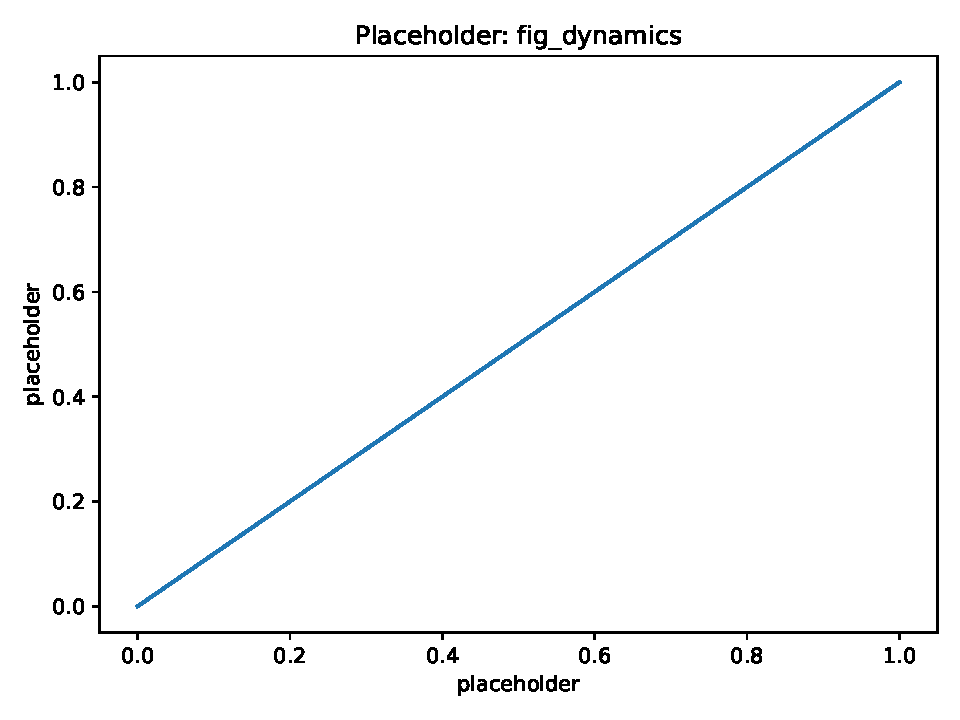
\includegraphics[width=0.95\linewidth]{artifacts/paper/fig_dynamics.pdf}
\caption{Training dynamics (validation Avg@8 vs. global step) for a
representative subset of methods.}
\label{fig:dynamics}
\end{figure}

\subsection{Stability and efficiency}
Table~\ref{tab:stability} aggregates stability and efficiency diagnostics.
Figure~\ref{fig:stability} visualizes the stability trade-off across methods.

\begin{table}[t]
\centering
\small
\begin{tabular}{lccc}
\hline
Method & Monotonicity $\uparrow$ & NDR $\downarrow$ & TTT $\downarrow$ \\
\hline
$\Delta L$ (best) & \textemdash & \textemdash & \textemdash \\
\textbf{CAPO--EB (best)} & \textemdash & \textemdash & \textemdash \\
\hline
\end{tabular}

\caption{Stability and efficiency diagnostics computed from validation curves.
Higher monotonicity is better; lower NDR and lower TTT are better.}
\label{tab:stability}
\end{table}

\begin{figure}[t]
\centering
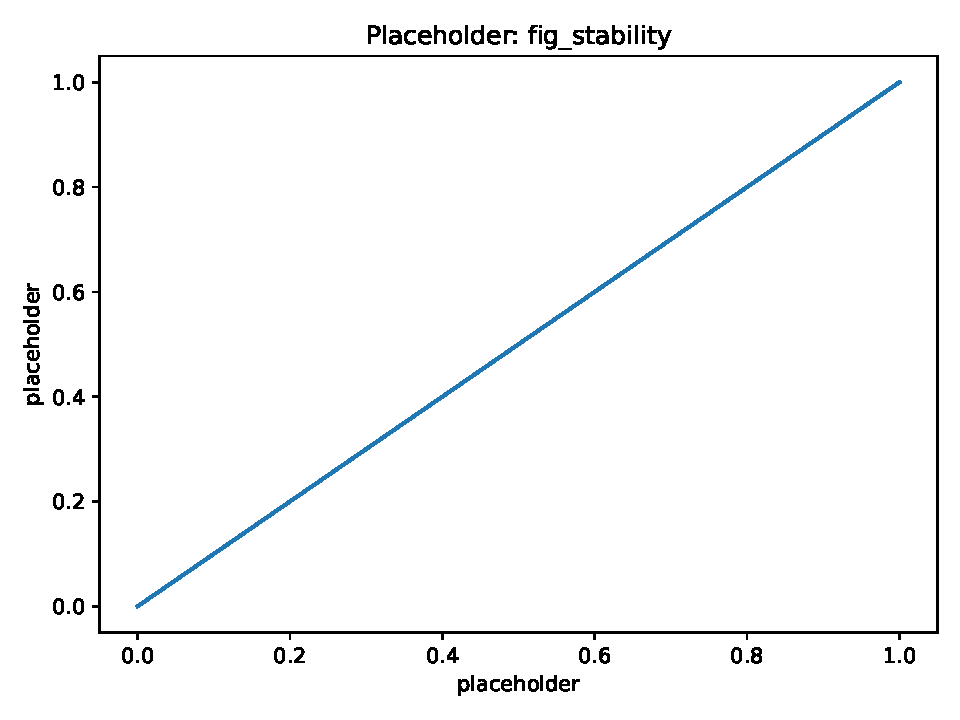
\includegraphics[width=0.95\linewidth]{artifacts/paper/fig_stability.pdf}
\caption{Stability summary. Each point corresponds to a method, plotted by
monotonicity (higher is better) and negative drift rate (lower is better).}
\label{fig:stability}
\end{figure}

\subsection{Length equity}
To make length effects explicit, we stratify validation by response-length
deciles and report verifier success within each stratum.

\begin{figure}[t]
\centering
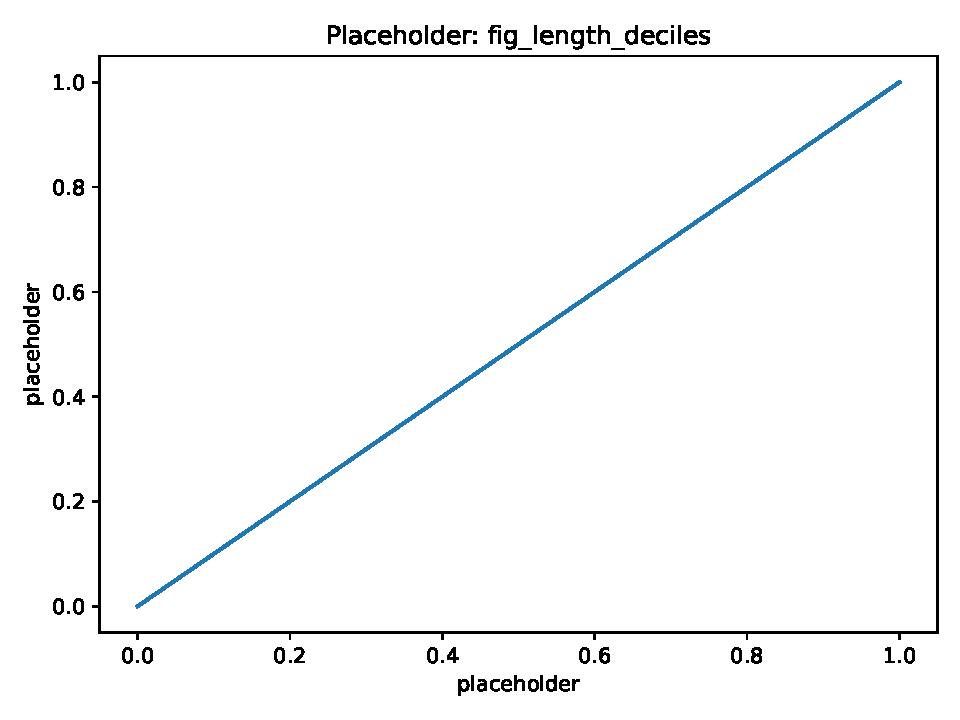
\includegraphics[width=0.95\linewidth]{artifacts/paper/fig_length_deciles.pdf}
\caption{Verifier success by response-length decile. This analysis highlights
whether a method disproportionately favors short (or long) trajectories even
when end-to-end accuracy is similar.}
\label{fig:length-deciles}
\end{figure}


\subsection{Additional diagnostics and failure modes}

\paragraph{Weight degeneracy.}
A central practical concern in any variance-based weighting scheme is \emph{degeneracy} of the normalized weights $w_i$:
if one trajectory receives nearly all mass, the effective number of trajectories contributing to the update collapses.
To monitor this, we recommend reporting the effective sample size
$\mathrm{ESS}:=(\sum_i w_i)^2/(\sum_i w_i^2)$ and/or the entropy $-\sum_i w_i\log w_i$ of the normalized weights.
CAPO includes explicit clipping and $\varepsilon$-regularization steps (Algorithms~\ref{alg:eb-lite}--\ref{alg:eb-capo}) to prevent pathological collapse.

\paragraph{Length-conditioned bias.}
Length-based normalization can introduce systematic differences in how short and long trajectories are reinforced.
The length-decile analysis in Figure~\ref{fig:length-deciles} is intended to expose such effects.
For publication-quality reporting, we recommend additionally stratifying by reward outcome (success/failure) and by prompt difficulty to distinguish genuine credit assignment from spurious length preferences.

\paragraph{Model misspecification.}
The variance law $v(L)\propto L^{\beta}s(L;\xi)$ is a working model.
When this model is misspecified, CAPO remains unbiased (because \eqref{eq:linear-agg} enforces unbiasedness), but suboptimal weighting can increase variance and exacerbate instability.
The robustness results in \S\ref{subsec:cs} and the covariance examples in Appendix~\ref{sec:eb-examples} provide guidance for diagnosing when simple dependence surrogates (e.g., exponential or compound-symmetry) are adequate.